% Chapter 4
\chapter{Xilinx Aurora 8B10B IP Core for high speed GTP interface}
\label{chapter4}
%--------------------------------------------------------------------------
\section {Overview}

As the communication speed increases to multi gigabyte, I/O performance decays and prevents successful functioning of the hardware. High speed parallel communication has many drawbacks like increase in number of required I/O on chip, increase in the hardware resource requirements, specialized I/O port design to support multi gigabyte communication, crosstalk etc.. Parallel communication also needs additional control lines to give meaning to the data for example enable, multiplexing data/control. On the other hand serial communication and clock recovery methods help overcome some of the issues like reduced hardware resource requirement, reducing inter wire crosstalk etc.. and in serial communication flags and markers are created to differential data and control signals.\\

The main components of any serial communication are serializer, de-serializer, and data/clock recovery blocks. These serialization and de-serialization blocks are realized by a few D flip-flops whereas the clock/data recovery block utilizes PLLs. The clock recovery process does not provide a common clock or send the clock with the data. Instead, a phased locked loop (PLL) is used to synthesize a clock that matches the frequency of the clock that generates the incoming serial data stream.\\

A VHDL evaluation platform and interface to the Xilinx Aurora 8B10B IP has been designed, tested and evaluated. The evaluation platform takes an arbitrary amount of data sources and sends the data over 1,2,4 or 8 multi-gigabyte serial lanes, using the Aurora 8B10B protocol. A lightweight communications protocol for point-to-point data transfer, error detection and recovery is used to maintain a reliable and efficient transmission scheme. The Aurora 8B10B IP is a lightweight protocol and transceiver interface for Xilinx FPGAs, based on the 8B10B line encoding protocol.

\section{Our Approach}

In our design we started with high speed serial I/O IP core ``Xilinx Aurora 8B10B \cite{AuroraManual}", along with a few other similar high speed serial communication IP cores like RapidI/O and SerialI/O but decided to test and use Aurora 8B10B. The Aurora core is a high-speed serial communication application developed based on the Aurora protocol for Virtex-5 FPGA GTP/GTX transceivers, Virtex-6 FPGA GTX transceivers, and Spartan-6 FPGA GTP transceivers. The core is an open-source code and supports both Verilog and VHDL design environments. This core can be generated by using Xilinx core generator details of generation given in Appendix A.1. This generated core comes with an example design that consists of a frame generator module and a frame check module. Frame generator module generates 16-bit data implemented using Linear Feedback Shift Register (LFSR) and which can be regenerated in frame check module for comparison. Aurora core has a local link layer block (explains in detail below) which is interfaced from these frame generator and frame check module. A detailed user guide provided by Xilinx explains the customization, generation and usage of the core. Figure \ref{Auroratop} shows a top level architecture of the aurora core. To use this core we need to understand the framing interface as shown in the Figure \ref{AuroraLocalLink} gives pin description.\\
\begin{figure}[H]
  \centering
   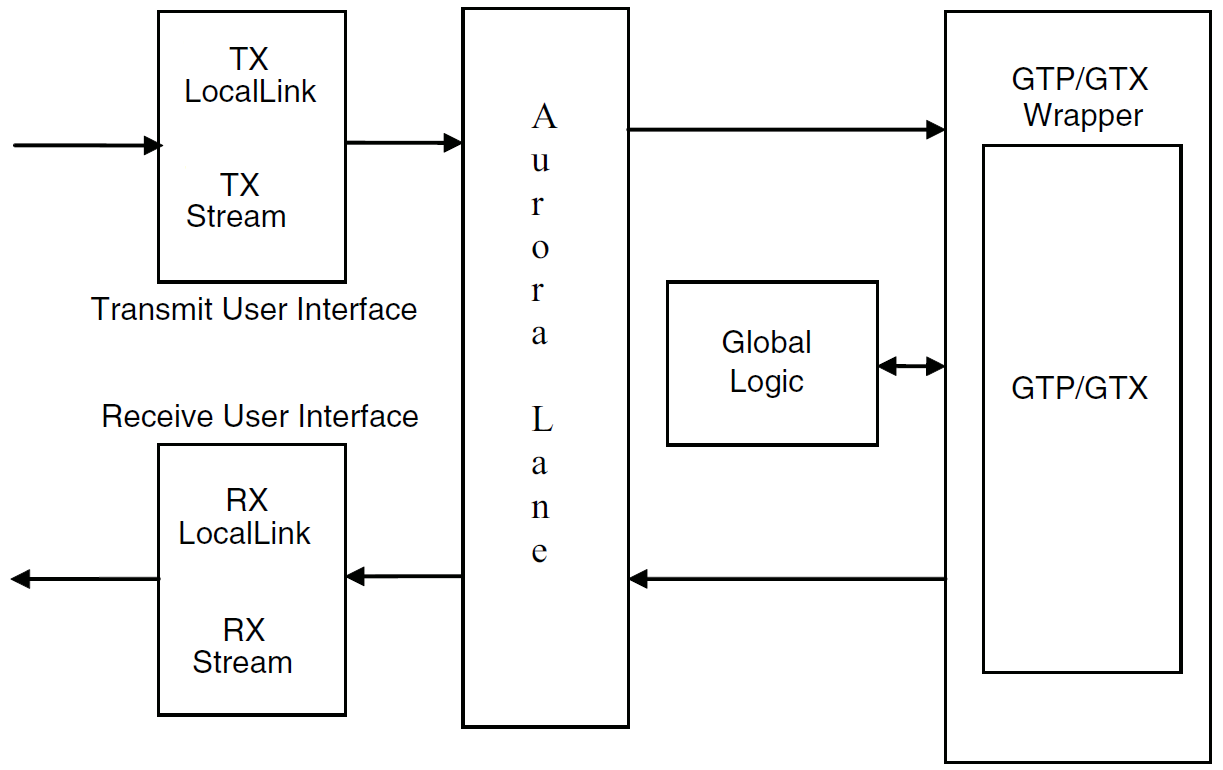
\includegraphics[scale=0.8]{./figs/auroraTop}
  \caption{\textbf{Aurora Top level Module Block Schematic \cite{AuroraManual}}}
  \label{Auroratop}
\end{figure}

To transmit data, the user manipulates control signals to cause the core to do the following:
\begin{itemize} 
	\item{Take data from the user on the TX\_D bus}
	\item{Encapsulate and sends the data across lanes in the Aurora 8B10B channel (TX\_SOF\_N, TX\_EOF\_N)}
	\item{Pause data (that is, insert idles) (TX\_SRC\_RDY\_N)}
\end{itemize}

When the core receives data, this interface performs the following steps:
\begin{itemize}
	\item{Detects and discards control bytes (idles, clock compensation, SCP, ECP)}
	\item{Asserts framing signals (RX\_SOF\_N, RX\_EOF\_N)}
	\item{Recovers data from the lanes}
	\item{Assembles data for presentation to the user on the RX\_D bus}
\end{itemize}

\begin{figure}[H]
  \centering
   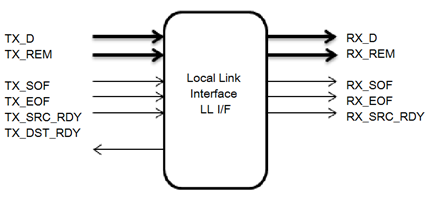
\includegraphics[scale=1]{./figs/auroraLocalLink}
  \caption{\textbf{Aurora Local Link Interface Pin Diagram\cite{AuroraManual}}}
  \label{AuroraLocalLink}
\end{figure}

Latency through an Aurora core is caused by pipeline delays through the protocol engine and through the GTP/GTX transceivers. The protocol engine pipeline delay increases as the Local Link interface width increases. The GTP/GTX transceivers delays are fixed per the features of the GTP/GTX transceivers. This section outlines expected latency for the Aurora 8B10B core's Local Link user interface in terms of USER\_CLK cycles for 2-byte-per-lane and 4-byte-per-lane designs. For the purposes of illustrating latency, the Aurora 8B10B modules partitioned into GTP/GTX transceivers logic and protocol engine logic implemented in the FPGA fabric. This latency figures do not take into account the length of the serial interface. Maximum latency for a 2-byte design from TX\_SOF\_N to RX\_SOF\_N is approximately 52.\\

In addition to operations described above, Aurora core interface contains special components such as the elastic buffers, whose role is to avoid buffer overflow/underflow which may occurs due to the frequency difference between sender and receiver, as serializer (transmitter) and de-serializer (receiver) are located on different boards and use different clock sources. Depending on the transceiver configuration and the clocking scheme used, I/O bit rate varies between 600Mb/s and 3.123 Gbps\cite{AuroraISE}. However these values are theoretical, and represent only the serial line bit-rates, and not the end-to-end bit rate.
The maximum data rate that can be obtained when using Aurora 8B10B with a reference clock of 156.25 MHz is 2.5 Gbps effectively if encoding decoding is not considered and 3.125 Gbps for 8B10B encoding/decoding. 

\section{Simulation Result}

This partitioned network with high speed serial links introduces a latency of 36 clock cycles which is trade of against the reduction of number of required IOs. Whereas in case of Quasi-SERDES link module latency is 10 clock cycles. The results as compared to earlier UART links are much better. Simulation waveforms in Figure \ref{AuroraSimulation} show the flit transmitted from node 1 and received at node 3.

\begin{figure}[H]
  \centering
   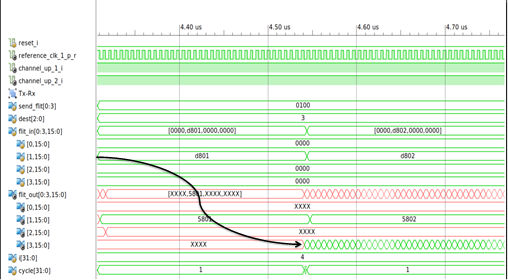
\includegraphics[scale=1]{./figs/AuroraSimulation}
  \caption{\textbf{Simulation Result of Aurora 8B10B integrated with 2 $\times$ 2 Mesh NoC}}
  \label{AuroraSimulation}
\end{figure}

\section{Advantages and Disadvantages discovered in usage of Aurora 8B10B}
\subsection{Advantages:}
\begin{enumerate}
	\item{Aurora 8B10B IP core is easy to generate and use in user design. The core generates with an example design which lowers designers manual integration effort.}
	\item{Aurora Core a light weight protocol with low resource requirements.}
	\item{The core is a scalable and flexible interface for communication set-up between two similar instances.}
	\item{Very high data rates can be obtained}
	\item{The IP core comes with an error checking mechanism with the design itself.}
	\item{The designer can work with the Aurora core without getting in great details of how the communication is actually happening}
\end{enumerate}


\subsection{Disadvantages:}
\begin{enumerate}
	\item{Aurora 8B10B IP core example design usage is not very resourceful}
	\item{Aurora Core need specialized hardware on chip that is GTP tiles which is device and vendor specific.}
	\item{In application like PG-NoC where a 7 $\times$ 3 interfaces has to be synthesized for partitioned NoC integrated with Aurora then on-chip GTP resources will be a limitation.}
	\item{Simulation results suggests that a GALS architecture would be difficult to implement as the clock rates for the interfaced modules needs to be synchronized.}
	\item{The IP core can not be used with any device and needs specialized high end board.}
	\item{A very large portion of the IP core is open source but beyond a point when GTP transceiver come into picture its not very clear what is happen and how is to communication happening.}
\end{enumerate}


With a few customizations, the Aurora IP seems like a good candidate to use instead of more complex and expensive serial protocols. The only drawback is the highly simplified user interface when generating the IP core. Many of the transceiver settings available are not present here. They have to be configured using another Core-gen wizard or manually changed in the generated VHDL files. Discovering the advantages and disadvantages we decided to design a simpler communication link specific to CONNECT type NoC which may not necessarily be a serial communication link. This link was developed as a general hardware block independent from the device on which its going to be used. We shall discuss this communication link and its simulation and implementation details in the next chapter.